\chapter{Applications}\label{Chapter:Applications}

\section{Local filters}

A local filter is an operation that computes a new image $g$ using as input the image $f$.
Each value $g(i,j)$ is computed with, typically, a few values of $f$ around the coordinate $(i,j)$.
Such operation is often referred to as a \textit{filter}, and the region over which the values of $f$ are considered is called the \textit{support} of the filter, and denoted $\partial_{i,j}$.
We denote $\overline{\partial_{i,j}}=\partial_{i,j}\cup(i,j)$ the support with the ``central'' coordinate.
The support may change from position to position, leading to \textit{adaptive filters}.
The operations may range from linear transformations to any computation over $\{f(k,\ell)\colon (k,\ell)\in\overline{\partial_{i,j}}\}$.

Listing~\ref{Code:Skeleton} provides a skeleton of the code for a general local filter.

\begin{lstlisting}[language=R,label=Code:Skeleton,frame=top,caption={Skeleton for local filters}]
Skeleton <- function(y, s) {

# Input: the image and the side of the squared support

# Output: filtered image z

# Input image dimensions
m <- dim(y)[1]
n <- dim(y)[2]

# Make space for the output image
z <- y

# Main loop
margin <- (s+1)/2
marginm1 <- margin-1
for(k in margin:(m-margin)) {
for(ele in margin:(n-margin)) {

  values <- y[(k-marginm1):(k+marginm1),(ele-marginm1):(ele+marginm1)]

  z[k,ele] = mean(values)
  }
}

return(z)
}
\end{lstlisting}

In this simple example we compute the mean, but this may be replaced by any computation.
Notice that the filter is only applied to the core of the image, i.e., to every pixel where the window fits.
The other pixels are left unfiltered.

In the following, we will see the effect of filters.

\subsection{Images and transects}

Figure~\ref{Image:Strips} shows a phantom that frequently appears in the SAR literature\cite{Petty:LAAR:ProtocoloLee}.
It consists of two classes: a background, and strips and dots of three different sizes.
This phantom can be turned into as many images as desired, using simulated data from any distribution.

\begin{figure}[hbt]
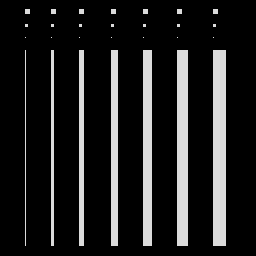
\includegraphics[width=.7\linewidth]{strips}
\caption{The \textit{strips} phantom}\label{Image:Strips}
\end{figure}

Figure~\ref{Image:Strips1LookExp} shows the result of adding single look noise in multiplicative fashion to the strips-and-dots image.
The background mean was set to $1$, and the rest to $5$.
The image is shown after equalization.

\begin{figure}[hbt]
	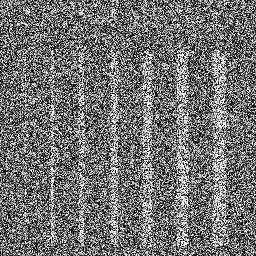
\includegraphics[width=.7\linewidth]{stripsExp1}
	\caption{The \textit{strips} phantom with exponential noise (after equalization)}\label{Image:Strips1LookExp}
\end{figure}

The effect of speckle is noticeable.
The small details, both the fine strip and the dots are now barely visible.

Figure~\ref{Plot:Transects} shows a horizontal and e vertical transect of both the phantom (in dark violet) and the observed (in violet) data.
The mean values ($5$ and $10$) are shown as dashed black lines.
This kind of representation is useful for checking the effect of filters around edges.

\begin{figure*}[hbt]
	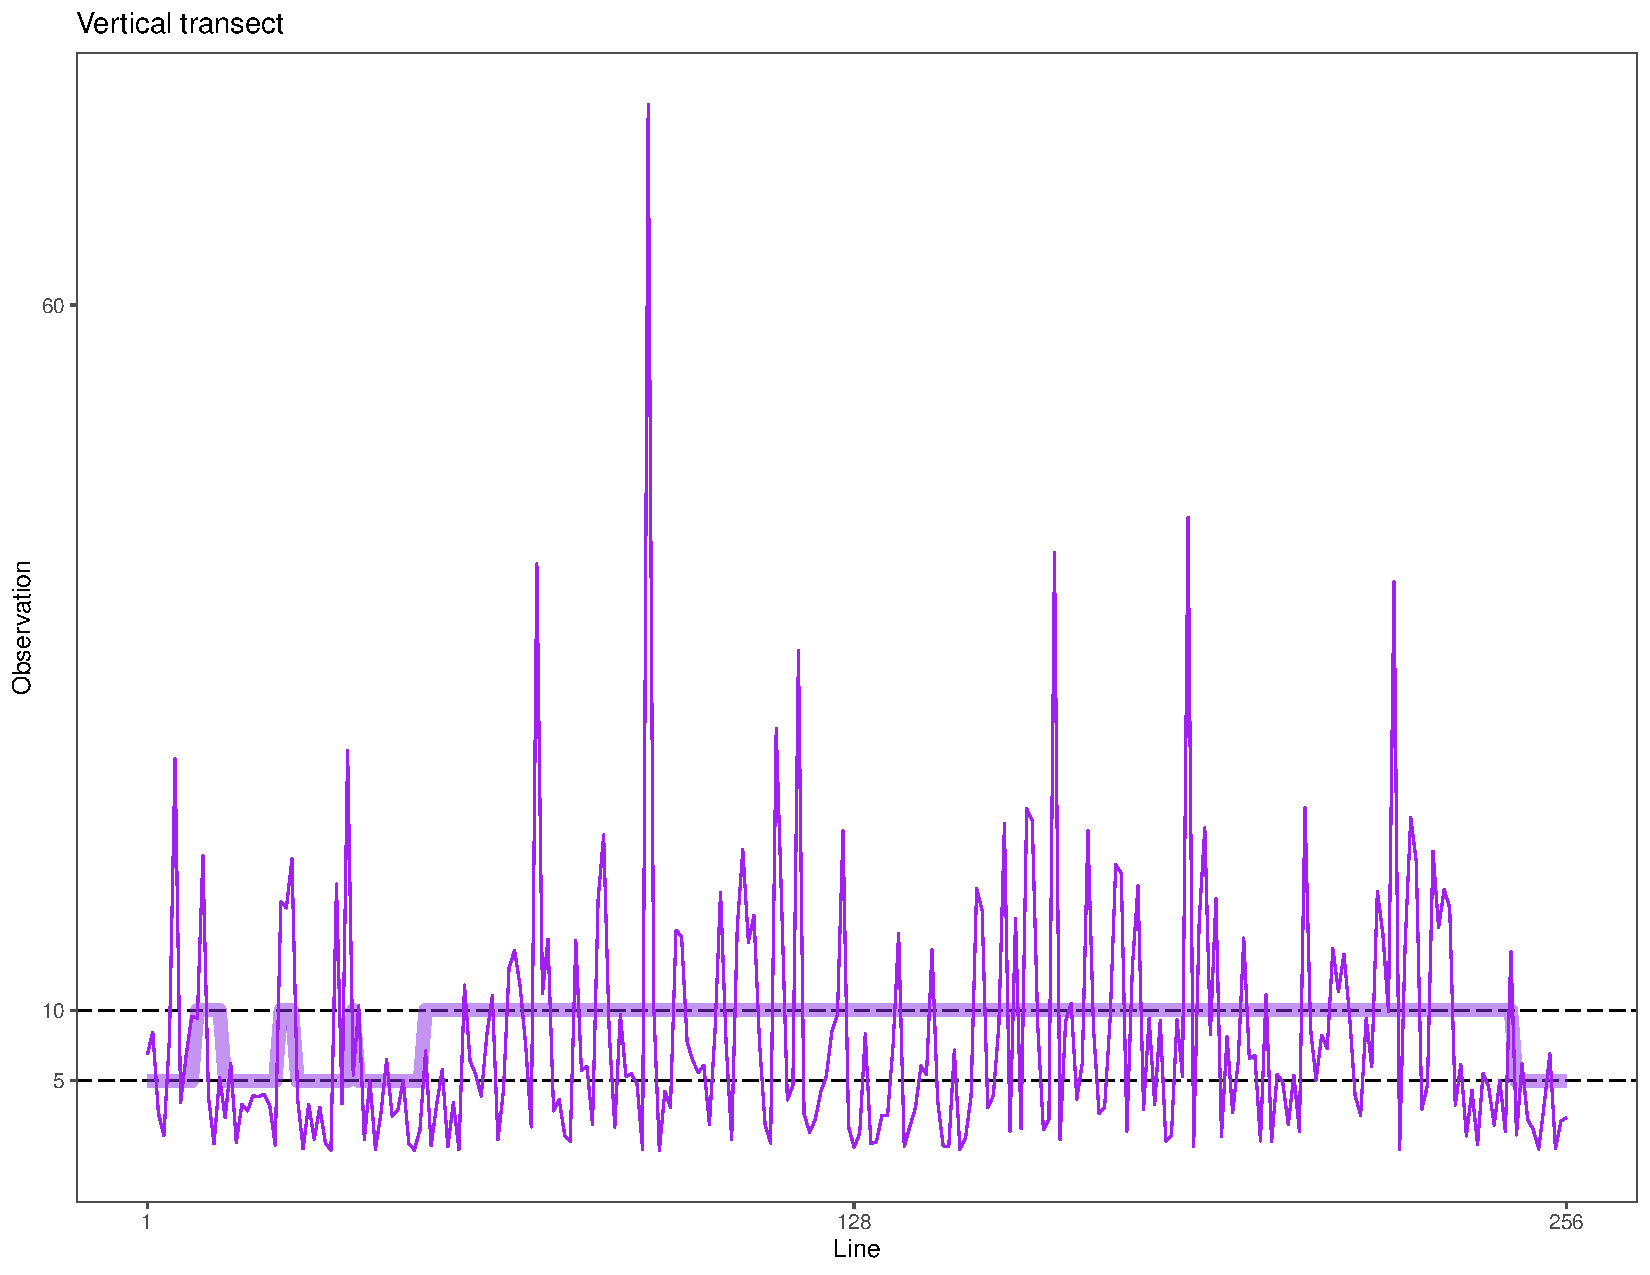
\includegraphics[width=.48\linewidth]{VerticalTransect}
	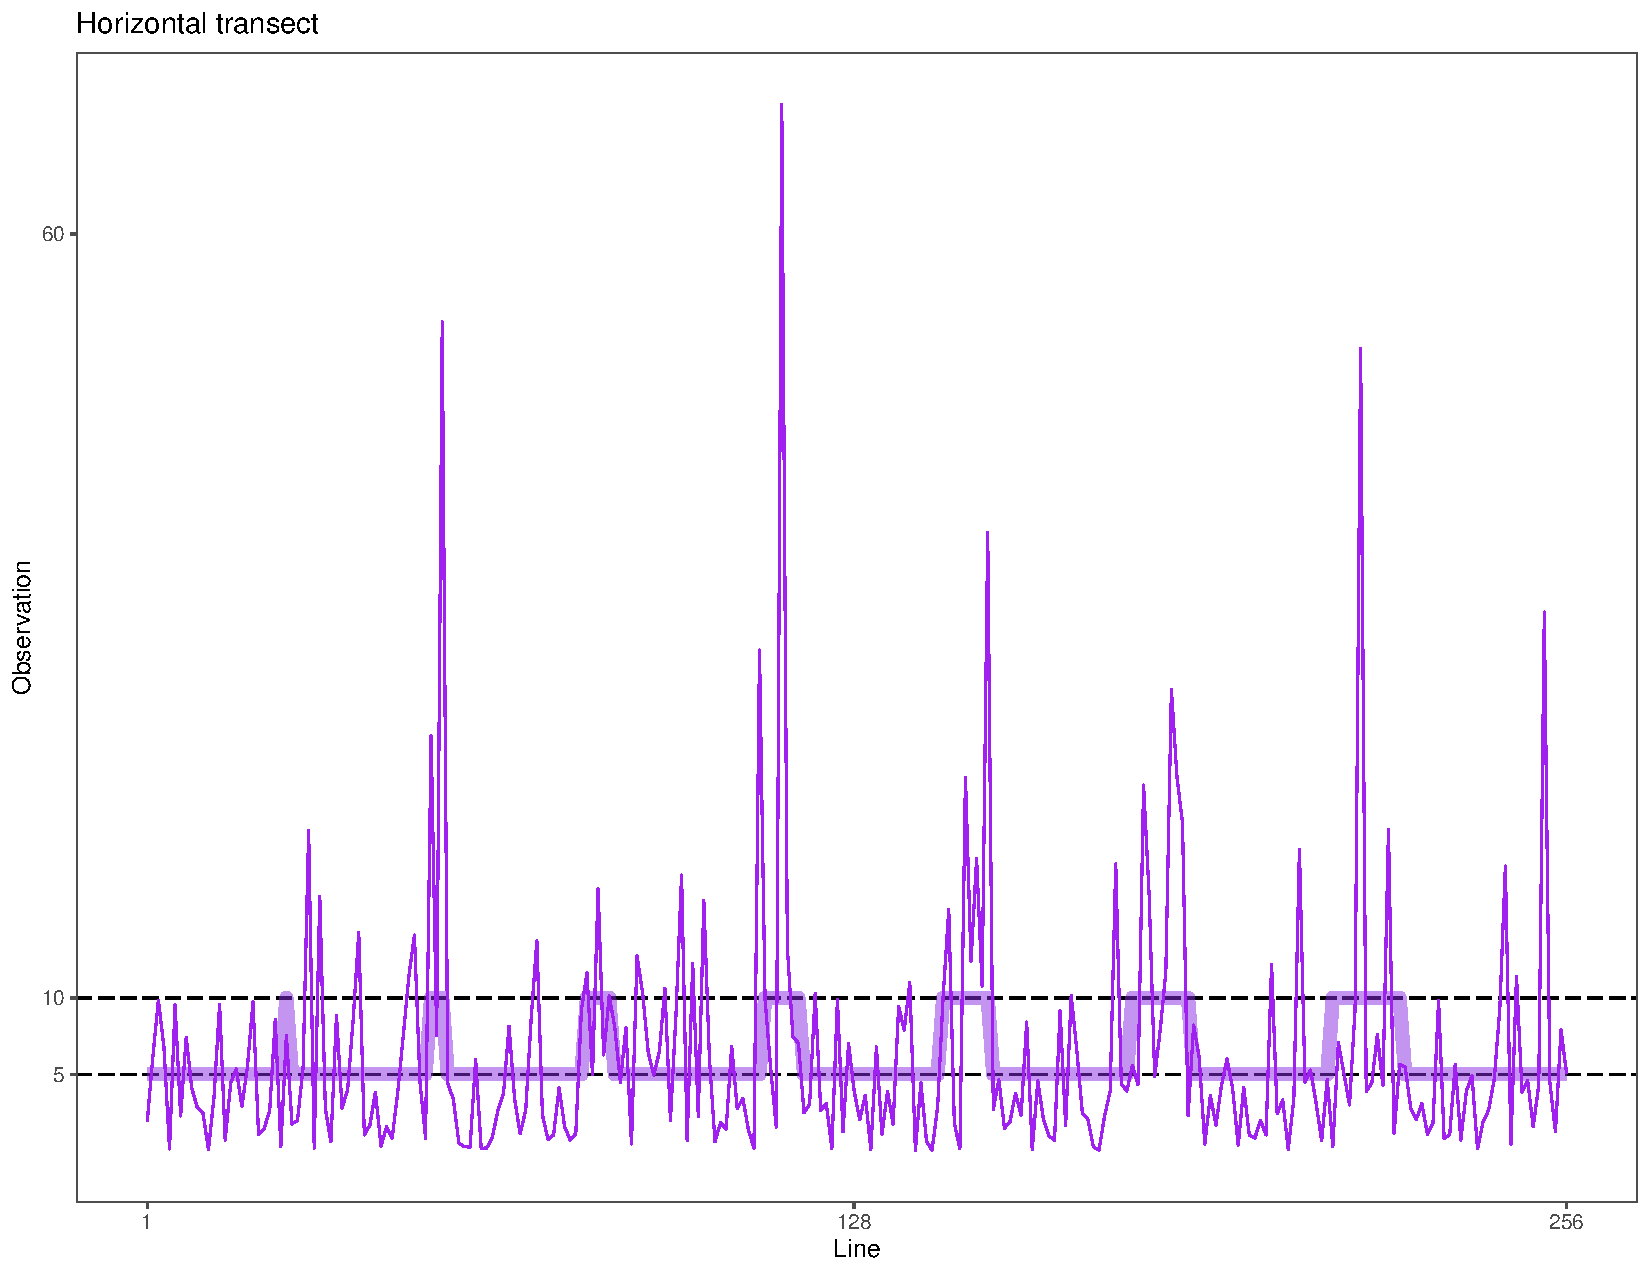
\includegraphics[width=.48\linewidth]{HorizontalTransect}
	\caption{Vertical (left) and horizontal (right) transects}\label{Plot:Transects}
\end{figure*}

Figure~\ref{Image:Exp1Mean} shows the results of applying the mean filter to the image shown in Fig.~\ref{Image:Strips1LookExp} with windows of sizes $3\times3$ and $7\times7$.
The noise in the new images has been reduced, but at the expense of blocking effect and loss of small details.

\begin{figure*}[hbt]
	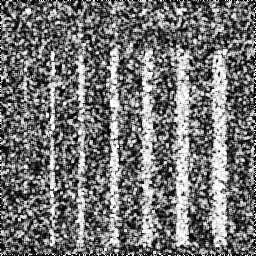
\includegraphics[width=.48\linewidth]{Exp1Mean3}
	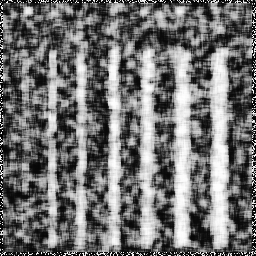
\includegraphics[width=.48\linewidth]{Exp1Mean7}
	\caption{Speckled strips filtered with the mean and windows of sizes $3\times3$ (left) and $7\times7$ (right)}\label{Image:Exp1Mean}
\end{figure*}

Figure~\ref{Image:Exp1Median} shows the results of applying the median filter to the image shown in Fig.~\ref{Image:Strips1LookExp} with windows of sizes $3\times3$ and $7\times7$.
The noise has also been reduced, also at the expense of blocking effect and loss of small details.

\begin{figure*}[hbt]
	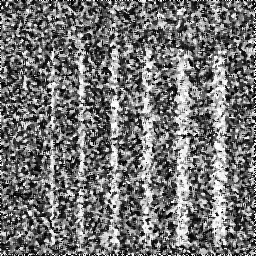
\includegraphics[width=.48\linewidth]{Exp1Median3}
	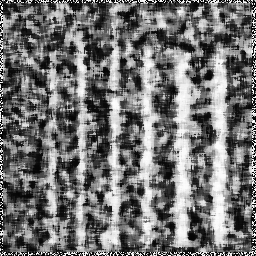
\includegraphics[width=.48\linewidth]{Exp1Median7}
	\caption{Speckled strips filtered with the median and windows of sizes $3\times3$ (left) and $7\times7$ (right)}\label{Image:Exp1Median}
\end{figure*}

The reader may notice that the blurring effect is smaller with the median than with the mean, mostly when applying the $7\times7$ window.
This desirable effect comes at a price: the noise is less reduced by the median than by the mean.